\documentclass[12pt]{article}
\usepackage{amsthm}
\usepackage{bbm}
\usepackage{amssymb}
\usepackage{mathtools}
\mathtoolsset{showonlyrefs,showmanualtags}
\usepackage{etoolbox}
% \usepackage{booktabs}
% \usepackage{url}
%\usepackage{setspace}
\usepackage[margin=1in]{geometry}
% \usepackage{authblk}
\usepackage{natbib}
% \usepackage[page]{appendix}
\usepackage[nomarkers,nolists]{endfloat}
\usepackage{graphicx}
% \usepackage{tikz}
% \usetikzlibrary{calc}
\usepackage{xcolor}
\usepackage{subfig}
\usepackage{enumitem}
% \usepackage{array} % tables with fixed width and alignment
\DeclareMathOperator{\AUC}{AUC}
\DeclareMathOperator{\V}{Var}
\DeclareMathOperator{\cov}{Cov}
\DeclareMathOperator{\corr}{Corr}
\DeclareMathOperator{\sd}{sd}
\DeclareMathOperator*{\argmax}{arg\,max}
\DeclareMathOperator*{\argmin}{arg\,min}
\DeclareMathOperator*{\diag}{diag}
\newcommand{\E}{E}
\renewcommand{\P}{P}
\newcommand{\cind}{\perp \!\!\! \perp}
\newcommand{\X}[1][]{X_{0#1}}
\newcommand{\Y}[1][]{X_{1#1}}
\newcommand{\W}[1][]{W_{#1}}
\newcommand{\w}[1][]{w_{#1}}
\newcommand{\z}[1][]{w_{#1}}
\newcommand{\D}[1][]{D_{#1}}
\renewcommand{\t}[1]{{#1}^T}
\renewcommand{\star}[1]{{#1}^\ast}
\newcommand{\infl}[1][]{\psi_{#1}}
\newcommand{\F}{F}
\newcommand{\G}{G}
% \newcommand{\D}{D}
\newcommand{\m}{m}
\newcommand{\n}{n}
\newcommand{\N}{m+n}
% \newcommand{\risk}{\rho}
\newcommand{\risk}[1][]{\rho_{#1}}
\newcommand{\auc}{\theta}
% \newcommand{\betastar}{\beta_0}
% \newcommand{\aucdiff}{\Delta\text{AUC}}
% \newcommand{\aucdiffhat}{\hat{\Delta\text{AUC}}}
\newcommand{\aucdiff}{\Delta\auc}
\newcommand{\aucdiffhat}{\Delta\hat{\auc}}
\newcommand{\kernel}[2]{\{#1 < #2\}}
% \newcommand{\infl}{\phi}
\newcommand{\h}{h}
\newcommand{\termb}{term 2 }
\newtheorem{theorem}{Theorem}
\newtheorem{proposition}[theorem]{Proposition}
\newtheorem{lemma}[theorem]{Lemma}
\newtheorem{corollary}[theorem]{Corollary}
\newtheorem{remark}[theorem]{Remark}
\theoremstyle{definition}
\newtheorem{example}{Example}%[section]
\newtheorem{subexample}{Example}%[section]
\makeatletter
% \def\input@path{{input/}{figs/}}
% \graphicspath{{./figs/}}
\newtoggle{commenttoggle}
\toggletrue{commenttoggle}
\newcommand{\comment}[1]{
  \iftoggle{commenttoggle}{
    {\normalsize{\color{red}{ #1}}\normalsize}
  }
  {}
}
\title{Nonparametric Estimation of the AUC of an Index with Estimated Parameters}
% \author[1]{Haben Michael}
% \author[2]{Lu Tian}
% \affil[1]{University of Massachusetts}
% \affil[2]{Stanford University}
\date{}

\begin{document}
\maketitle
% ((previously: ``auc of an estimated index'' but that isn't actually the target of estimation))

Abstract. We describe a nonparametric method of estimating the AUC of
an index $\t\beta x$ when $\beta$ is estimated from the same data, with a
focus on nonparametric estimation of the difference of the AUCs of two
distinct indices.

\section{Introduction}

The AUC is a standard measure of how effectively a marker
discriminates between two classes. The difference in AUCs, written $\aucdiff$,
is a standard comparison of the discrimination of two markers.

In the medical sciences, the marker is often a linear combination
$\beta$ of a set of subject characteristics $x$. We refer here to
$\t\beta x$ as an ``index'' and its AUC as an ``index AUC.''
In medical fields, comparison of markers often takes the form of comparing two sets of
patient characteristics $x$ and $y$, with indexes $\t\beta x,\t\gamma y$. The
characteristics are often nested, $x\subset y$, as when investigating
the impact on discrimination of additionatal factors $y \backslash
x$. The difference in AUCs has been described by experts as
one of the most widely used measures of discrimination \citep{demler2017}. \comment{should be ``difference'' in discrimination I think?}

% biomarkers--index auc. often
% one index is based on a subset of covariates on which the other is based.

A related way of measuring the impact of additional covariates is to
directly compare the coefficients $\beta$ and $\gamma$ under a
model. The result of this comparison may conflict with the comparison
of AUCs. A series of papers in the 2010s noted the ``baffling'' and
``perplexing'' contradictions between the two methods, calling into
question the validity of $\Delta$AUC \citep{seshan2013}\comment{johnny cite}. While the
source of the contradiction was soon identified, remedies have been
slower to
arrive.% unexpected behavior when comparing $\aucdiff$ to tests on the indexes
% themselves. maybe mention ``bafflement'' over test behavior. at the
% begining of 2010s.

We present here a partial remedy, a method to nonparametrically
estimate $\aucdiff$ under the assumption that $\aucdiff\neq 0$.\comment{is
this the right characterization of the null?}
\comment{
useful cites: 
maybe cite seshan counts of clinical papers, sas proc. ((
seshan 2013: In the first four months of 2011 alone, we easily
identified seven articles in clinical journals that used the AUC test
to compare nested logistic regression models [11, 12, 13, 14, 15, 16,
17]))
}

\section{Background/setting}\label{section:background}


% difference of 2 aucs.
% may be viewed as a U-statistic.

An observation is modeled as a pair of covariates and a binary status indicator,
\begin{gather}
  \begin{aligned}\label{model:iid}
  (\W,\D), \W\in\mathbb{R}^p, \P(\D=0)=1-\P(\D=1)\in (0,1).
\end{aligned}
\end{gather}
Denote by $\X\sim\F,\Y\sim\G$ the RVs and
distributions obtained by conditioning $\W$ on $\D=0$ and $\D=1$.  We use ``control'' and ``case'' generically to refer to these conditional RVs and distributions. Let
$(\W[1],\D[1]),\ldots,(\W[\N],\D[\N]),$ be an IID sample under \eqref{model:iid}, with the
class variables
\begin{align}
  \X[1],\ldots,\X[\m] \overset{IID}{\sim} \F,   \Y[1],\ldots,\Y[\n] \overset{IID}{\sim} \G, \m=\sum\{\D=1\}, \n=\sum\{\D=0\}
\end{align}
% Based on this data, analyst obtains coefficients $\beta,\gamma$.
% \comment{is $X=W|D=0$ or $=W\{D=0\}$?}
Vectors $\hat\beta \in \mathbb{R}$ and $\hat\gamma \in \mathbb{R}$ are
obtained based on the sample by some means%  we refer to generically as the
% ``coefficient estimation procedure''
. They are assumed to have finite
probability limits $\star\beta$ and $\star\gamma$ as
$\m,\n\to\infty$ under this procedure.

The AUC, measuring how effectively a scalar marker discriminates
between two classes, is the probability the maker associated with one
class is less than a stochastically independent marker associated with
the other class. A non-parametric estimator is the sample proportion
of markers in one class less than the markers in the other. In the
case that the markers are indexes with esimated coefficient
$\hat\beta$, the estimator is
\begin{align}
   \frac{1}{\m\n}\sum_{i,j}\kernel{\t{\hat\beta}\X[i]}{\t{\hat\beta}\Y[j]}.\label{defn:auchat}
\end{align}
The difference of index AUCs is  estimated nonparametrically by
\begin{align}
  \aucdiffhat=\frac{1}{\m\n}\sum_{i,j}\kernel{\t{\hat\beta}\X[i]}{\t{\hat\beta}\Y[j]}
  -  \frac{1}{\m\n}\sum_{i,j}\kernel{\t{\hat\gamma}\X[i]}{\t{\hat\gamma}\Y[j]} . \label{defn:aucdiffhat}
\end{align}
In applied settings, an explicit probabilty model may not be
specified, and often the estimation methods for $\hat\beta$ and
$\hat\gamma$ imply inconsistent
models (see Example \ref{example:diff:parametric}). % E.g., logistic models with nonzero covariates omitted from the
% reduced model
 Nevertheless inference is
sought \comment{cite applied papers}, particularly 1. whether the difference
in the AUCs of the two markers $\t{\hat\beta} x$ and
$\t{\hat\gamma} x$ is in some limiting sense nonzero, and if so 2. the
magnitude of the difference. Assume here that limiting sense is the
difference of AUCs of the indexes at the starred parameters,
so the target of inference is%$\t{\star\beta} x$ versus $\t{\star\gamma} x$:
\begin{align}
  % \aucdiff=\frac{1}{\m\n}\sum_{i,j}\kernel{\t{\star\beta}\X[i]}{\t{\star\beta}\Y[j]}
  % -  \frac{1}{\m\n}\sum_{i,j}\kernel{\t{\star\gamma}\X[i]}{\t{\star\gamma}\Y[j]} .
  \aucdiff=\P(\t{\star\beta}\X[i]<\t{\star\beta}\Y[j])
- \P(\t{\star\gamma}\X[i]<\t{\star\gamma}\Y[j]).\label{defn:aucdiff}
\end{align}
% For fixed $\hat\beta,\hat\gamma$, 

The statistic \eqref{defn:aucdiffhat} may be viewed as a U-statistic process with
two-sample kernel
$(x,y)\mapsto \kernel{\t\beta x}{\t\beta y} - \kernel{\t\gamma x }{
  \t\gamma y}$, indexed by $\beta,\gamma$, and evaluated at the random
vectors $\hat\beta,\hat\gamma$. This statistic presents two
complications for an analysis using basic U-statistics theory.

1. Under the null of no difference, $\aucdiff=0$, the statistic
\eqref{defn:aucdiff} is often a degenerate U-statistic. The asymptotic
distribution of a degenerate U-statistic is a weighted combination of
chi-squares, with weights depending on the distributions of the
obesrvations. In the case of the difference of index AUCs, estimators
have been presented only in a few specific cases, e.g., \citet{heller2017}, and the
null distribution for common coefficient estimation method such as
logistic regression remains ``intractable''
\citep{lee2021}.% ((heller)) gives the asymptotic null distribution
% specifically in the case that the coefficient estimation procedure is
% the MRC ((ref below)).
% [[update: heller doesnt make modeling
% assumptions on the covariates, only on the estimation of betahat;
% maybe that is a benefit over testing risk function? ie is there a test
% for the mrc coefficients that doesnt require modeling covariates?]]
% ((demler))  assuming coefficents are esitmated by lda with gaussian
% covariates.
% recently noted ((cite)) that asy null distribution remains
% intractable for common estimation methods eg logistic regression.

% \comment{mention demler 2012 as another indirect approach, like pepe?. Indirect approaches to testing the null have been proposed. demler, pepe.}

Instead, the literature has proposed the use of more covenient testing
problems equivalent in certain settings to the testing
$\aucdiff=0$. \citet{demler2011} show that when the covariates are
Gaussian and the coefficient estimation procedure is LDA, the null is
the same as testing for equality of the Mahalonobis distance between
the two class distrbutions. An F-test, valid in finite samples, may
therefore be used instead of testing the AUC directly.
\citet{pepe2013} describe a more general
approach. % provides a more uniform approach to the problem of testing
%  for zero difference between nested index aucs. The authors suggest a more
% convenient often equivalent testing problem.
The risk function for a binary RV $\D$ based on a set of covariates
$\W\in\mathbb{R}^p$, $\risk[\W]:\mathbb{R}^p\to\mathbb{R}$, is the
function $\z \mapsto \P(\D=1 \mid \W=\z)$. Let
$(\D[0],\W[0],\W[0]'),(\D[1],\W[1],\W[1]')$ be IID. The authors show
that the null of equal AUCs of the risks,
\begin{align}
  &\P(\risk[{\W,\W'}](\W[0],\W[0]') < \risk[{\W,\W'}](\W[1],\W[1]') \mid \D[0]=0,\D[1]=1)\\
  &=
  \P(\risk[{\W}](\W[0]) < \risk[{\W}](\W[1]) \mid \D[0]=0,\D[1]=1)
\end{align}
holds if and only if the risk functions are equal,
$\risk[{\W,\W'}]=\risk[\W]$. Often the coefficient
estimation procedure is of secondary importance and the goal of
testing the null $\aucdiff=0$ is to test if certain additional
covariates improve discrimination. In this case, the test may be based
on the risks instead. Even if interest lies in testing for the
difference in AUCs where $\hat\beta,\hat\gamma$ are obtained through a
particular estimation procedure, e.g., logistic
regression, % Suppose it is needed to test
% $P(\beta^T(x,y)|D=0 < \beta^T(x,y)|D=1)=P(\gamma^Tx|D=0 <
% \gamma^Tx|D=1)$, obtained by LDA, logistic regression etc.
for many estimation procedures there is a monotone link connecting the limiting index to the risk,
e.g., the expit function (see Example \ref{example:auc:glm}). Since the AUC is invariant to monotone
transformations, the risk may still be used to test for a
difference. % Provided the coefficient
% estimation model is correct, the two models, reduced and full, are compatible under the
% null, since then $\star\beta=\star\gamma$, 
% so that testing if there is some monotone
% link $h$ such that
% $P(D=1|x,y)=h(\beta^T(x,y)),P(D=1|x)=h(\gamma^T(x))$, then the test is
% the same as
% $P(risk(x,y)|D=0 < risk(x,y)|D=1)=P(risk(x)|D=0 < risk(x)|D=1)$ so one
% may just test $risk(x,y)=risk(x)$. 

A drawback to this approach is it requires knowing the true risk
function. If the null distribution of $\aucdiffhat$ were available,
one might directly compare the discrimination of the indices
$\t{\hat\beta} \W$ and $\t{\hat\gamma} \W$, and possibly use the
indices in practice, without knowing the correct risk
function. However, unless computing the null distribution of the
$\aucdiffhat$ calls for fewer modeling assumptions, improved efficiency,
or some other advantage, may as well test risk functions.

As we don't offer any such improvements over testing the risk, we only consider
the alternative case $\aucdiff\neq 0$ in the remainder.

2. A second issue is that $\hat\beta,\hat\gamma$ are estimated from
the data, so that the observations on which the statistic \eqref{defn:aucdiffhat} is based
are not IID. Non-degenerate U-statistics with estimated parameters are
typically still normal though estimation of the parameter may affect
the asymptotic distribution. This issue is addressed in the remainder.

% ((maybe mention that nolan-pollard papers address both problems in
% almost the same setting (degree 2 ustats) but still need to
% nonparametrically compute the liiting chi squared distribution for the
% null))

\section{Method}\label{section:method}


The usual approach to finding the asymptotic distribution of
a non-degenerate U-statistic, which we adopt, is to find an asymptotically equivalent IID average, to which
the CLT can be applied.


For control and case distributions $F,G$ on $\mathbb{R}^p$ and vector $\beta$, denote the AUC of the index, $P(\t\beta X < \t\beta Y)$ for a control $X\sim F$ and independent case $Y\sim G$, by
\begin{align}
  \auc(F,G,\beta) &= \int\kernel{\t\beta x}{\t\beta y}dF(x)dG(y).
\end{align}
With this notation,
$\aucdiffhat=\auc(\hat\F,\hat\G,\hat\beta)-\auc(\hat\F,\hat\G,\hat\gamma)$.
We write each of the two terms of the difference as an IID average, and later take the difference to
represent $\aucdiffhat$ as an IID average. Decompose the centered estimate
$\auc(\hat\F,\hat\G,\hat\beta)- \auc(\F,\G,\star\beta)$ as a sum of two
terms, reflecting the two sources of estimation, the AUC estimation
and the coefficient
estimation,%, the CDFs $\hat\F,\hat\G,$ and the parameter $\beta$.
\begin{align}
  &\auc(\hat\F,\hat\G,\hat\beta) - \auc(\F,\G,\star\beta)\\
  &=\auc(\F+\delta\F,\G+\delta\G,\star\beta+\delta\beta) - \auc(\F,\G,\star\beta+\delta\beta) \label{method:delong term}\\
    &+ \auc(\F,\G,\star\beta+\delta\beta)-\auc(\F,\G,\star\beta)\label{method:adjustment term}
\end{align}
Where $\delta\F=\hat\F-\F,$ etc.

Term \eqref{method:delong term}: As the function $\auc(\cdot,\cdot,\beta)$ is bilinear,
\begin{align}
  &\auc(\F+\delta\F,\G+\delta\G,\star\beta+\delta\beta) - \auc(\F,\G,\star\beta+\delta\beta)\\
  &=\auc(\delta\F,\G,\star\beta+\delta\beta)+\auc(\F,\delta\G,\star\beta+\delta\beta)+\theta(\delta\F,\delta\G,\star\beta+\delta\beta).\label{method:term 5 expansion}
\end{align}
The third and final term in \eqref{method:term 5 expansion} is an average of $\m\n$ uncorrelated terms and therefore $o(n^{-1/2})$.%  $o((\N)^{-1/2})$, % $\theta(\delta\F,\delta\G,\beta+\delta\beta)=o(n^{-1/2})$:
% \begin{align}
%   &\P(\theta(\delta\F,\delta\G,\beta+\delta\beta)>(\N)^{-1/2}\epsilon) \\
%   &\le \P(\int d|\F_n-\F|(x) > (\N)^{-1/4}\sqrt\epsilon)+\P(\int d|\G_n-\G|(x) > (\N)^{-1/4}\sqrt\epsilon)\to 0
% \end{align}
% by a DKW-type bound.
% ((Pf: By multivariate DKW (e.g., Serfling p.61), $\P(|\F_n-\F|_\infty > n^{-1/4})<c\exp(-c\sqrt n)$))
% ..((in case this approach doesnt work, can just cite nolan--pollard approach))

% The first two terms, partially expected and for fixed $\beta+\delta\beta$, are IID
% averages.  To account for the randomness in $\beta+\delta\beta$ expand in a Taylor series % if differentiable at $\beta$ ((always differentiable for $\beta\neq 0$?)),
% \begin{align}
%   ...
% \end{align}
% and if sufficiently smooth, can interchange derivtive and expectation
% \begin{align}
%   ...=0
% \end{align}
% since $\E(...)=0$ for all $\beta\neq 0$.

% ((generally not smooth at $\beta=0$, auc kernel jumps))

For fixed $\star\beta+\delta\beta$, the first two terms are centered IID averages
That the randomness in $\delta\beta$ is asymptotically negligible at the $\sqrt {\N}$ rate,
$$
\auc(\delta\F,\G,\star\beta+\delta\beta)+\auc(\F,\delta\G,\star\beta+\delta\beta)
=\auc(\delta\F,\G,\star\beta)+\auc(\F,\delta\G,\star\beta) + o((\N)^{-1/2}),
$$
follows from empirical process theory, in particular ``stochastic
equicontinuity'' of the empirical processes $\beta \mapsto \auc(\delta\F,\G,\beta), \beta \mapsto \auc(\F,\delta\G,\beta)$ \citep{pollard1984}. %Consequently term 1 ((ref)) is % ((need to discuss derivative of hajek term at starred parameter being 0))))

Therefore,
\begin{align}
  % &\auc(\F+\delta\F,\G+\delta\G,\beta+\delta\beta) - \auc(\F,\G,\beta+\delta\beta)\\
  &\auc(\F+\delta\F,\G+\delta\G,\star\beta+\delta\beta) - \auc(\F,\G,\star\beta+\delta\beta) \\%+ o((\N)^{-1/2})\\
  &=-\frac{1}{\m}\sum_{i=1}^\m(1-\G(\t{\star\beta}\X[i])-\auc(\F,\G,\star\beta)) + \frac{1}{\n}\sum_{i=1}^\n(\F(\t{\star\beta}\Y[i])-\auc(\F,\G,\star\beta))+ o((\N)^{-1/2})\\
    &=\frac{1}{\N}\sum_{i=1}^{\N}\left(-\frac{\{\D[i]=0\}}{\P(\D=0)}(1-\G(\t{\star\beta}\W[i])-\auc(\F,\G,\star\beta)) + \frac{\{\D[i]=1\}}{\P(\D=1)}(\F(\t{\star\beta}\W[i])-\auc(\F,\G,\star\beta))\right)\\
  &+ o((\N)^{-1/2}) \label{method:hoeffding}
\end{align}
% ((last line doesnt maintain the $1/n$ rate? nvm it does--factor out
% the clsas probability estimate and end up with the product of two
% averages)) 
This IID representation is known as the
Hoeffding decomposition of a U-statistic, and is the same as the first
von Mises derivative. % Represents term \eqref{method:delong term}
The CLT may be applied to get the asymptotic distribution of
$\aucdiffhat$ in situations that the term \eqref{method:adjustment term} is
negligible, e.g., if $\hat\beta=\beta$ were not estimated (see Section \ref{section:examples}
for additional scenarios when \eqref{method:adjustment term} is
negligible)). The approach of \citet{delong1988} in such situations is to estimate
$\F,\G$ above using the empirical CDFs $\hat\F,\hat\G$,
giving rise to the standard Delong statistic for inference on the
$\aucdiff$,
\begin{align}
  -\frac{1}{\m}\sum_{i=1}^\m(1-\hat\G(\t{\beta}\X[i])-\auc(\hat\F,\hat\G,\beta)) + \frac{1}{\n}\sum_{i=1}^\n(\hat\F(\t{\beta}\Y[i])-\auc(\hat\F,\hat\G,\beta)).
\end{align}



Term \eqref{method:adjustment term}: Assume
$\sqrt{n}(\hat\beta-\star\beta)\to 0$ in probability,
$\beta\mapsto\auc(\F,\G,\beta)$ is differentiable at $\star\beta$. Let
the function $\infl[\hat\beta]$ represent the estimator $\hat\beta$ as
an IID mean
\begin{align}
  \hat\beta-\star\beta=(\N)^{-1}\sum_{i=1}^{\m+\n}\infl[\hat\beta](\W[i]) + o((\N)^{-1/2})
\end{align}
i.e., $\infl[\hat\beta]$ is an influence function for the $\hat\beta$. Then \eqref{method:adjustment term} is
\begin{align}
  &\auc(\F,\G,\beta+\delta\beta)-\auc(\F,\G,\beta)  \\
  &=(\hat\beta-\star\beta)\frac{\partial}{\partial\beta}\auc(\F,\G,\beta) + o_P((\N)^{-1/2})\\
  &=\frac{\partial}{\partial\beta}\auc(\F,\G,\beta)(\N)^{-1}\sum_{i=1}^{\m+\n}\infl[\hat\beta](\W[i]) + o_P((\N)^{-1/2}).
\end{align}

Putting the two parts together,
\begin{align}
  &\auc(\hat\F,\hat\G,\hat\beta) - \auc(\F,\G,\beta)\\
  &=\frac{1}{\m+\n}\sum_{i=1}^{\m+\n}\left(-\frac{\{\D[i]=0\}}{\P(\D=0)}(1-\G(\t{\star\beta}\W[i])-\auc(\F,\G,\star\beta)) + \frac{\{\D[i]=1\}}{\P(\D=1)}(\F(\t{\star\beta}\W[i])-\auc(\F,\G,\star\beta))\right) \\
  &+ \frac{\partial}{\partial\beta}\t{\auc(\F,\G,\beta)}\sum_{i=1}^{\m+\n}\infl[\hat\beta](\W[i]) + o_P((\N)^{-1/2}) \label{method:iid representation}
\end{align}
\comment{maybe combine into one sum}

\begin{proposition}\label{proposition:auc} Given a sample
  $(\W[1],\D[1]),\ldots,(\W[\N],\D[\N])$ as \eqref{model:iid}, and estimator
  $\hat\beta$ based on the sample.
  Assumptions:
  \begin{enumerate}
  \item available influence function for
    $\hat\beta$
  \item $P(\D=0) \in (0,1)$
  % \item 
  \item   $\auc(\F,\G,\cdot)$ is differentiable at $\star\beta$
  \end{enumerate}
  Assertion:
  $(\N)^{-1/2}(\auc(\hat\F,\hat\G,\hat\beta)-\auc(\F,\G,\star\beta))$
  is asymptotically normal with mean zero and variance given by the
  variance of a term in \eqref{method:iid representation}. This variance may be consistently
  estimated as $\sqrt{\N}$ times the sample variance of the terms in
  \eqref{method:iid representation}.
\end{proposition}
Take the difference with the same representation of another estimator,
$\auc(\hat\F,\hat\G,\hat\gamma)$, to obtain an IID representation of
$\aucdiffhat$.

\begin{corollary} \label{corollary:delta auc}  Given a sample
  $(\W[1],\D[1]),\ldots,(\W[\N],\D[\N])$ as \eqref{model:iid}, and estimators
  $\hat\beta, \hat\gamma$ based on the sample. Assumptions:
  \begin{enumerate}
  \item Assumptions of Proposition \ref{proposition:auc} apply to $\hat\beta,\hat\gamma$ both
  \item $\star\beta\neq\star\gamma$
  \end{enumerate}
  Then $(\N)^{-1}(\aucdiffhat-\aucdiff)$ is
asymptotically normal with mean zero and variance given by a term in
the difference of IID means \eqref{method:iid representation}.  This variance may be consistently
estimated as $\sqrt{\N}$ times the sample variance of the difference of terms as in \eqref{method:iid representation}
\end{corollary}
% REMARKS ((to be removed))

% - Benefits of approximating by an iid sum:

% 1. ((remove)) As above, can de-couple the two terms of the difference $\aucdiff$ and treat
% estimation the auc of an index using an estimated index.


% \begin{remark}
It isn't required that $\hat\beta$ be estimated by a correctly
specified model, only that it has some probability limit at the
parametric rate.  Though the procedure for obtaining the estimate
$\hat\beta$ and the associated influence function $\infl$ often
involve some parametric assumptions, we still term the procedure
described here as ``non-parametric'' since the estimator in
Proposition \ref{proposition:auc} is valid under misspecification of
the coefficient model. Whatever the estimation procedure is it will be
known to the analyst, so that an influence function may be chosen, if
one exists.
% \end{remark}
% ((all of these o(n) expressions should be o(m+n) ))...
% ((influence function should be average not sum))

% adding the two parts term-wise gives an iid representation of $\auc(\hat\beta)$:


What goes wrong under the null? If $\star\beta=\star\gamma$ then the
main terms in the Hoeffding-type decomposition
\eqref{method:hoeffding} cancel when the difference is taken, leaving
a term of order $o((\N)^{-1/2})$. Moreover the derivatives in
\eqref{method:adjustment term} are the same. In many situations where the index
is derived from a well-specified model the derivative is $0$ for at
least one of the two AUCs being differenced. In that case
\eqref{method:delong term} will also be $o((\N)^{-1/2})$, and $\aucdiffhat$
will degenerate under the usual $\sqrt{\N}$ normalization. The
condition $\star\beta\neq\star\gamma$ is just sufficient. It is
possible that in e.g. a nested logistic model both full and reduced
are misspecified, the Hoeffding term degenerates, the derivative
vanishes at neither $\star\beta$ nor $\star\gamma$, the influence
functions of $\hat\beta$ and $\hat\gamma$ differ, and then the limit
of $\aucdiffhat$ is still normal. \comment{check. also check against demler
2017 iff conditions for degeneracy.}

\comment{restructure--the above two paras are more like remarks. first 1 maybe goes to an estimation section.}

% ((use of starred parameter inconsistent in this section... drop it
% here in favor of $\delta\beta$ ?))
\section{Estimation}
% estimation section: discuss estimation of derivative, can be slow
% rate. so important that only need consistent estimator.
% \comment{simulaiton should mention estimated parameters, discuss influence function supplied}

Using Proposition \ref{proposition:auc} for non-parametric inference
will usually require certain parameters to be estimated. As mentioned
in Section \ref{section:method}, even if the coefficient beta were not
estimated, the terms in the estimator corresponding to the Delong
statistic would still require estimating the CDFs. In the adjustment
term, the influence function and derivative term will often require
estimated parameters.
% Application of the is an IID sum, and the sd estimate is the empirical
% estimator. This is itself an estimate of $\sqrt{\N}\hat\theta$, not
% $\hat\theta$.
Substituting consistent etimated parameters into the IID average is usually
asymptotically negligible as long as the dependence is continuous,
though of course  the efficiency of the
convergence may be affected. Non-parametric estimation of the derivative term, in
particular, is often slower than the usual parametric rate as it
requires estimating a random function in an interval.

% efficiency of asy convergence. % as long as the parameter estimates are
% consistent and dependence is continuous. of course may affect
% efficiency of asy convergence. %  The influence function may contain
% % nuisance parameters as long as it depends on them continuously and
% % consistent estimators are available.
% ((Just as the standard Delong estimator estimates the conditional CDFs
% $\F,\G$ using empirical CDFs))

% ((estimation section)) convergence to 0 of the non-delong part can be slow. even on simple
% data like iid gaussian covariates with a null logistic model.



\section{Examples}\label{section:examples}
\comment{add linear regression to collapsibility?}

Section \ref{section:method} decomposes the statistics $\hat\auc$ and
$\aucdiffhat$ as a sum of two terms
\eqref{method:delong term}, \eqref{method:adjustment term}. The first
corresponds to the estimation of the AUC by a U-statistic. The second
is an adjustment term corresponding to the use of estimated
coefficients. At times the adjustment vanishes in the limit, and the
estimtion of the coefficient may be ignored. In this case the usual
Mann-Whitney U-statistic, in the case of $\hat\auc$, or the Delong
statistic, in the case of $\aucdiff$, may be used for asymptotic
inference, provided of course the AUCs are distinct, as discussed in
Section \ref{section:method}.  When the adjustment term does not
vanish, Proposition \ref{proposition:auc} may be used for asymptotic
inference.

We give examples of data and models where coefficient estimation may
and may not be ignored when carrying out asymptotic inference on the
index auc.

\subsection{No effect of coefficient estimation}
In the ordinary course, the coefficient estimation can be ignored in
computing the index of a smooth AUC iff its derivative is 0 at the
probability limit of the coefficient,
$\partial_3\auc(F,G,\star\beta)=0$ in the notation of Section
\ref{section:method}. For the difference of two AUCs, the derivative
of each must usually be 0 at the respective coefficient probability
limits,
$\partial_3\auc(F,G,\star\beta)=\partial_3\auc(F,G,\star\gamma)=0$.

\subsubsection{AUC}\label{section:examples:auc}

We first give examples where the coefficient estimation may be ignored in estimating the AUC of an index.

\begin{example}[Estimator: MRC, covariate restrictions:
none/nonparametric]\label{example:auc:mrc} The maximum rank correlation method of computing
the coefficients is
\begin{align}
  \hat\beta = \argmax_{\beta:|\beta|=1} \auc(\hat\F,\hat\G,\beta).
\end{align}
The method is non-parametric. By construction the empirical AUC is
stationary at the coefficient estimates, and under regularity
conditions the AUC $\auc(\F,\G,\beta)$ is stationary at the probability limit $\star\beta$, as well.
\end{example}

While the MRC is a nonparametric maximizer of
$\beta\mapsto\auc(\F,\G,\beta)$, it may also happen  under parametric models that the derivative vanishes
at the probability limit of the coefficient vector. The following proposition, highlighted
by \citet{mcintosh2002}, \citet{pepe2013}, furnishes a class of
examples.  For two real functions of $\W$, $f_1$ and $f_2$, let the
relation $f_1\sim_{(\W,\D)} f_2$ hold iff $f_1(\W)$ has the same conditional
distribution given $\D$ as a strictly increasing function of
$f_2(\W)$, i.e., there is a strictly increasing function
$h:\mathbb{R}\to\mathbb{R}$ such that
$P(f_1(\W)<w|\D=i)=P(h\circ f_2(\W)<w|\D=i)$ for all $w\in\mathbb{R}$
and $i=0,1$.

\begin{proposition}
  Given a random vector $(\W,\D)$, $\W$ continuous, $\D$ binary, with
  index AUC $\auc(\F,\G,\cdot)$. Then,
\begin{enumerate}
\item The ROC curve of classifying $\D$ based on a real function of $\W$
is maximized pointwise by the likelihood ratio
$w\mapsto f_{\W\mid\D=1}(w)/f_{\W\mid\D=0}(w)$,\comment{cond desnities not defined}  equivalently, the risk of $\D$ based on $\W$, $\risk[{\W}](\cdot)$.

\item The AUC of a real function $f$ of $\W$ is maximal iff $f\sim_{(\W,\D)} \rho_{\W}$.
% 3. if deriv is concave,

\item Given a coefficient estimate $\hat\beta$ with probability limit $\star\beta$, if $\auc(\F,\G,\cdot)$
  is differentiable at $\star\beta$, and
  $\t{\star\beta}\W\sim_{(\W,\D)} \risk[\W](\W)$,\comment{slight abuse of $\sim$ notation here} then $\auc(\F,\G,\hat\beta)$ and
  $\auc(\F,\G,\star\beta)$ have the same asymptotic distribution.
\end{enumerate}
\end{proposition}
\begin{proof}
  \begin{enumerate}
  \item The first claim is an application of the Neyman-Pearson Lemma,
    as pointed out by \citet{pepe2013}\comment{ check if she did it
      first. swets.}. Let an FPR value $\alpha\in (0,1)$ be
    given. Viewing $\D$ as a parameter, the most powerful level
    $\alpha$ test of the null $\D=0$ versus the simple alternative
    $\D=1$ based on $\W$ rejects for large values of the likelihood
    ratio of $(\W,\D)$, i.e.,
    $f_{\W\mid\D=1}(W)/f_{\W\mid\D=0}(W)$. Therefore, the value of the
    ROC curve of the likelihood ratio at $\alpha$, which is the power
    of the Neyman-Pearson test, is maximal. Since the ROC curve is the
    same for increasing functions of the likelihood, and the risk is
    the expit of the log likelihood, the same holds of the risk.
  
  \item Though markers not related by an increasing function may have the
  same AUC, since the ROC curve of the risk is maximal, an index with
  the same AUC must have the same ROC curve. The latter does imply the
  index has the same conditional distributions as an increasing
  function of the risk.
\end{enumerate}
\end{proof}

\begin{example}[Coefficient estimator: any non-zero estimate,
  covariate restrictions: A single covariate] When there is a single
  covariate, $p=1$, the $\beta$ in \eqref{defn:auchat},
  for $\beta\neq 0$, cancels and the requirement is simply that the
  risk be increasing in the sole covariate, i.e., that the covariate
  or its negation be a risk
  factor.% ((ref simulations in demler 2017, where reduced model has a
% single covariate)).
\end{example}

\begin{example}[Parametric models where index is monotonically related
  to the risk]\label{example:auc:glm} The derivative will vanish in smooth parametric models
  under which the index is monotonically related to the risk
  function.% is
 % sufficient. %may also be necessary if deriv is concave.
\counterwithin{subexample}{example}
\begin{subexample}[Coefficient estimator: binary response MLE, covariate
restrictions: GLM link]\label{example:auc:glm} A prominent example where the index is an
increasing function of the risk is the index model for a binary
response:
\begin{align}
  \P(\D=1\mid\W=\w) = \h(\t\beta \w), \beta\in\mathbb{R}^p.
\end{align}
The function $\h$ is strictly increasing, such as a probit link,
logistic link, identity, etc.
\end{subexample}


\begin{subexample}[Coefficient estimator: LDA, covariate restrictions:
  multivariate Gaussian]\label{example:auc:lda} With $\W\mid\D=i\sim N(\mu_i,\Sigma),i=1,2$,
  the LDA estimate of $\beta$ has probability limit
  $\star\beta=\Sigma^{-1}(\mu_1-\mu_0)$. The likelihood ratio
  $f_{\W\mid\D=1}(w)/f_{\W\mid\D=0}(w)$ is an increasing function of
  $\t{(\mu_1-\mu_0)}\Sigma^{-1}w=\t{\star\beta}w$. That derivative
  vanishes also follows by taking $\Sigma_0=\Sigma_1$ in the upper bound given by Proposition
  \ref{proposition:lda}.
\end{subexample}

\begin{subexample}[Coefficient estimator: LDA, covariate restrictions:
  independent exponential family covariates with mean
  parameters, etc.]\label{example:auc:exponential} Let component $i$ of $\W$,
  $i=1,\ldots,p$, have conditional density given $\D=j,j=1,2$, of the
  form $h_i(w)\exp(\theta_{ij}w-A_{ij})$. If the components
  are independent, the likelihood ratio then satisfies
\begin{align}
  % \frac{f(w\mid \D=1)}{f(w\mid \D=0)} \sim \sum_{i=1}^n(\theta_{i1}-\theta_{i0})^tx_i
   \frac{f(w\mid \D=1)}{f(w\mid \D=0)} \sim \t{(\theta_1-\theta_0)}w
\end{align}
With the usual LDA estimators, $\star\beta={\star{\Sigma}}^{-1}\Delta\star{\mu}$, where $\Delta\star{\mu}=A_1'-A_0'$ and $\star\Sigma$ is diagonal with entries $\pi_0A_{i0}''+\pi_1A_{i1}'',i=1,\ldots,p, \pi_0=1-\pi_1=\P(D=0)$. If 1. the population variances are equal, $\pi_0A_{i0}''+\pi_1A_{i1}''$ doesn't depend on $i$, and 2. $\theta_i$ is the mean $A_i'$, then $\t{\star{\beta}}w \sim \t{(A_1'-A_0')}w \sim \risk[\W](w)$.
% \begin{align}
%   \hat\beta \to_p ...
% \end{align}
% and the index at probability limit is $...$. If 1. the covariates have the same population variances, say $\pi_0A_0''+\pi_1A_1''$, and 2. the parameter $\theta_{ij}$ is the mean $A_{ij}$, then
% \begin{align}
%   \beta x \sim \sum_{i=1}^n(A_{i1}'-A_{i0}')x_i \sim \risk (x)
% \end{align}
This application of LDA is not justified under the usual
homoskedasticity assumption, as the parameter $\theta_j,j=1,2,$ may
affect the variance across classes. It turns out the coefficient
estimation still does not affect the asymptotic distribution of the index AUC.
\end{subexample}
\end{example}

With gaussian data as in Example \ref{example:auc:lda} but unequal
class variances, or heteroskedastic exponential family data as in
\ref{example:auc:exponential} but non-independent covariates, the
derivative of the AUC coefficient limit need not vanish, as shown by
the example in Section \ref{section:lda}.

\subsubsection{Difference of AUCs}
Next we consider application of the examples given in Section \ref{section:examples:auc} to two AUCs computed from the same data, as when
computing the difference.

\begin{example}
  For a non-parametric estimator like MRC, Example \ref{example:auc:mrc}, there
  is no further difficulty. Each estimation procedure leads to a
  vanishing derivative. This example is discussed in \citet{heller2017}.
\end{example}
\begin{example}Likewise, there is no difficulty when one coefficient
  is estimated by a well-specified parameric estimator and the other
  by a non-parametric estimator, or e.g.  the single covariate case
  where there is effectively no estimator. % full
% model well-specified and reduced model a single covariate 
See, e.g., Fig. 1 in \citet{demler2017} and the corresponding simulation.
\end{example}

% To apply this example as justification for inference based on the
% standard Delong statistic requires that both AUC models be
% well-specified. In the case of comparing a full $...$ to a reduced
% model $...$.


\begin{example}[Parametric models]\label{example:diff:parametric} Next suppose both coefficient vectors being compared are modeled
  parametrically, and consider specifically nested binary response
  models \ref{example:auc:glm}.  First, if neither the full model nor the
  reduced model is well spcified, there is no reason to expect the
  derivative to vanish by virtue of \ref{example:auc:glm}
  and in general coefficient estimation must be accounted for. Second,
  if the reduced model is well-specified, then comparison with a
  superset of the covariates will generally lead to the null
  situation, i.e., a degenerate U-statistic, as discussed in Section \ref{section:background}.
% if the full well-specified, reduced not, vice
% versa, and both misspecified. If neither is correctly specified,
% require accounting for derivative term. if reduced model is correct,
% then full model is.
Finally, suppose that the full model is well-specified, e.g., when the full
model contains a superset of the model covariates, and the reduced
model a strict subset of the fuller set. \comment{give citations to
simulations/data anlayses} In many cases correctness of the full
model,
\begin{align}
    \P(\D=1\mid(\W,\W')=(\w,\w')) = \h(\t\beta (\w,\w')), \text{ for some }\beta\in\mathbb{R}^{p+q}\label{defn:binary response}
\end{align}
implies the reduced model cannot be correct
\begin{align}
  \P(\D=1\mid \W=\w)=\E(\h(\t\beta (\w,\w'))\mid \w)\neq \h(\t\beta \w) \text{ for any }\beta\in\mathbb{R}^p.\label{examples:diff:collapsing}
\end{align}
As a result the derivative term contributed by the reduced set AUC will be nonzero and must be
accounted for.
% In the case of comparing a
% correctly specified full model $\P(D=1)=...$ to a reduced model $...$,
For the binary response model, the requirement is that the
marginalization does not break the model, i.e., the inequality in
\ref{examples:diff:collapsing} is an inequality for some $\beta$ in
the reduced model coefficient space. This condition is somewhat
different from ``collapsibility,'' the requirement that the
coefficients belonging to the remaining covariates be the same after
integrating out an independent set of covariates.  Some examples where
this condition holds are:
% and it often
% will not be the both will be well specified. excpet collapsible models,
% where the derivative is 0 in both models and therefore--assuming
% correct specification--can just use the basic delong stat, ignoring
% estimation of aprameters.

% need to check derivative 0 and also model assumptions.


% 2. full model well specified, implying reduced model also well
% specified. ie the true covariates only need be a subset of those
% available.
\counterwithin{subexample}{example}

\begin{subexample}[Coefficient estimator: probit regession, covariate
  restrictions: Gaussian] When $h$ in \eqref{defn:binary response} is
  the standard normal CDF and the covariates are multivariate
  Gaussian, the marginalized model respects the probit link.% \comment{not the same as collapsibility since marginalized covariates need not be independent of remaining, and reduced coefs need not be the same}
\end{subexample}

% \begin{subexample}[Coefficient estimator: logistic regression, covariate restrictions: Gaussian mixture, etc.] as covariates in the special case that beta is the lda/malanobis dist beta. This example is almost the same as the homoskedastic LDA example, since [[ref fisher lda display]] the posterior probabilities are given by ... . 
% \end{subexample}

When $h$ is the logistic function, and logistic regression is used to
estimate the coefficients, the marginalized risk is not generally a
logistic function of the index. Several authors have suggested,
however, that the coefficient estimation may be ignored
\citep{demler2011} \comment{give citations. is this the right demler
  paper?}. In fact, as shown in forthcoming work \comment{or add to
  appendix?}, for whatever link $h$, if the covariates are gaussian,
then the adjustment term vanishes, and coefficient estimation may be
ignored, only when the covariates under the marginalized model are the
covariates that would be obtained under a probit model. Though the
derivative may not vanish, however, it may be negligible, so that in
practice the coefficient estimation may be ignored. A heuristic reason
to expect a small adjustment term is that the logistic risk
are often close to the probit risk, where the adjustment does
vanish.

% \begin{subexample} [Coefficient estimator: logistic regression,
%   covariate restrictions: Gaussian with block diagonal covariance]
%   With Gaussian covariates, when the covariates in the reduced set are
%   uncorrelated with the remaining covariates, the derivative of the
%   AUC at the reduced set coefficient probability limit
%   vanishes. Though the Gaussian assumption is too strong for many
%   applications, the block diagonal variance condition may not
%   be. Often when testing the discrimination of additional covariates,
%   the effect of the currently used covariates are regressed out. This
%   case is discussed in \comment{((forthcoming)).need to rework this
%   example..deriv small but not zero. idea: with probit+gaussian the gradient is 0. any nonzero amount is therefore attributable to the difference between explit and normal CDF.}
% \end{subexample}
\begin{subexample} [Coefficent estimator: LDA, covariate restrictions:
  Gaussian] When the full model is a well-specified Gaussian LDA model
  \ref{example:auc:lda}, the reduced model will be as well. This
  example is discussed in \citet{demler2011} \comment{give their
    mahalanobis distance characterization. cite other papers that discuss this model} and considered further in Sections \ref{section:lda} and \ref{section:simulation}. LDA models are collapsible
  more generally, but the index may not be an increasing function of
  the risk/likelihood without the Gaussian assumption.  % Though LDA is
  % not usually regarded as an example of a binary response model, it is
  % included here as an example of a model compatible with
  % marginalizing.
\end{subexample}
\end{example}

% ((maybe cite bridge distribution
% paper.))
% adam at applestore cambridge, say chris at customer rleations said to call

% examples where derivative is 0:
% 1. single covariate. with a single predictor the derivative will often be zero, bc the risk
% (where the derivative of the auc is 0), $r(x)$, is often a monotonic
% function of $x$, and
% $P(\beta x_0 < \beta x_1) = P(x_0 < x_1) = P(r(x_0) < r(x_1))$ in this
% case. Demler 2017 uses a single covariate in the reduced model, so
% their example doesn't say much.
% % 2. exponential family (see notes)



\subsection{Coefficient estimation affects inference}\label{section:lda}
Next we describe a situation where estimation of the coefficient must be
accounted for when conducting inference on the difference of AUCs or
even just a single AUC. The setting is a misspecification of the
parametric model \ref{example:auc:lda} where, but for the
misspecification, coefficient estimation would not affect the
asymptotic distribution. The nonparametric estimator provides the
requires adjustment missing from the basic Delong estimator, and may
therefore be viewed as a robust estimator.

Suppose Gaussian linear discriminant analysis is applied to estimate
the coefficient vector but the model is possibly misspecified in that
the two classes may not have the same covariance. The model is:
\begin{gather}
  \begin{aligned}\label{model:heteroskedastic lda}
    \W | \D=d \sim \F_i=N_p(\mu_i,\Sigma_i), d=1,2\\
    \P(\D=1)=1-P(\D=0)=\pi_1
  \end{aligned}
\end{gather}
The LDA parameter estimation procedure is to base class membership on
the sign of $\t{\hat\beta} x$, where
  \begin{align}
    \hat\beta&=\hat{\Sigma}^{-1}(\hat\mu_1-\hat\mu_0)\\
    \hat\mu_1-\hat\mu_0&=\n^{-1}\sum_i\Y[i] - \m^{-1}\sum_i\X[i]\\
    \hat\Sigma &= \m/(\N)\sum_i(\X[i]-\hat\mu_0)\t{(\X[i]-\hat\mu_0)} + \n/(\N)\sum_i(\Y[i]-\hat\mu_1)\t{(\Y[i]-\hat\mu_1)}
  \end{align}
  An intercept is usually computed when carrying out LDA but may be
  ignored here since the AUC is invariant to shifts. The LDA parameter
  estimates, under the unmet assumption of a common variance for the
  two classes, tend in probability to
  \begin{align}
    \star\beta &={\star{\Sigma}}^{-1}(\mu_1-\mu_0)\\
    \star\Sigma &= \pi_0\Sigma_0+\pi_1\Sigma_1
  \end{align}
  Let
  $\Sigma=(\Sigma_0+\Sigma_1)/2,\Sigma_\pi=\pi_0\Sigma_0+\pi_1\Sigma_1$.
  The index AUC and its partial derivative with respect to the
  coefficient are
  \begin{align}
    \auc(\F,\G,\beta) &= \Phi\left(\frac{\t\beta\Sigma_\pi\beta}{\sqrt{2\t\beta\Sigma\beta}}\right)\\
    \frac{\partial}{\partial\beta}\auc(\F,\G,\beta) &= \phi\left(\frac{\t\beta\Sigma_\pi\beta}{\sqrt{2\t\beta\Sigma\beta}}\right)\frac{\t\beta}{\sqrt{2}(\t\beta\Sigma\beta)^{3/2}}
                                                      ((\t\beta\Sigma_0\beta)\Sigma_1-(\t\beta\Sigma_1\beta)\Sigma_0).
  \end{align}
  The derivative is $0$ at $\star\beta$ iff
  $(\t\beta\Sigma_0\beta)\Sigma_1\beta=(\t\beta\Sigma_1\beta)\Sigma_0\beta$
  for $\beta=\star\beta$, equivalently, $\star\beta$ is an eigenvector
  of $\Sigma_0^{-1}\Sigma_1$. For example, if the
  covariates are independent with a common variance, $\Sigma_d\propto I$, the derivative will be 0. As a second example, if $\Sigma_0\propto\Sigma_1$, then $\Sigma_0^{-1}\Sigma_1\propto I$ and again the derivative vanishes. % In terms of the
  % Gaussian parameters, the condition is that $\Delta\star\mu$ be an
  % eigenvector of $\Sigma\Sigma_\pi^{-1}$. 2 examples: 1. independent
  % data, ((...)), 2. proportional covariance matrices. 
  The first example is already implied by the general exponential
  family result in Example \ref{example:auc:exponential} above but not the second as the
  observations are not independent.
  % show that derivative term can be unbounded. % must consider also
  % variance of infl function ie inverse fisher information, i.e., the
  % components of  % It is possible for $\auc'(\F,\G,\star{\beta})$ to have large
  % % components which are countered by variance of the parameter
  % % estimates. 
  Even when the derivative is large, its effect may be mitigated. When
  $\Sigma\approx\star\Sigma$, the derivative term is approximately
  $O(|\Sigma|^{1/2})$, whereas the influence function is approximately
  $O(|\Sigma|^{-1/2})$, the root of the inverse Fisher information, so
  that the product, giving the entire adjustment term, is
  approximately $O(1)$.

  As the imbalance between the classes increases, the size
  $|(\star{\Sigma})^{-1} \auc'(\F,\G,\star{\beta})|$ of the adjustment
  term may grow, as show in Proposition \ref{proposition:lda}.
  % \begin{align}
  %   % \Sigma_0 = \diag(\epsilon\cdot\mathbbm{
  %   \Sigma_0=\begin{pmatrix}
  %     \ddots & & & &\\
  %     & \epsilon & & & &\\
  %     & & \ddots & & &\\
  %     & &  & 2-\epsilon& &\\
  %     & &  & & \ddots&
  %   \end{pmatrix}
  %   \Sigma_1=I,
  %   \beta=\sqrt{2/p}\mathbbm{1}
  % \end{align}
  % Then
  % $|(\star{\Sigma})^{-1} \auc'(\F,\G,\star{\beta})| \to \pm \infty
  % \mathbbm{1}$ as $\pi_0 \to 1$ and $\epsilon\to 0$ simultaneously.
  One therefore expects that under this scenario inference based on the Delong estimator will be faulty, as verified by simulation in Section \ref{section:simulation}. % ((possible to give result so that the sign of the derivative term is controlled, so that delong can be forced either to low fpr or low power?))
  
  %Results summarized and extended:
  
  \begin{proposition}\label{proposition:lda} Let $(\W,\D)$ follow \eqref{model:heteroskedastic lda}, with full rank conditional covariance matrices $\Sigma_d, d=0,1$. Then,
    \begin{enumerate}
\item The adjustment term satisfies
  \begin{align}
    sd(\frac{\partial}{\partial\beta}\auc(\F,\G,\beta)\infl[\hat\beta](\W[i])) &= |\Sigma_{\pi}^{-1/2}\frac{\partial}{\partial\beta}\auc(\F,\G,\beta)|\\
    &\le |\pi_1-\pi_0|/(2\sqrt\pi)\frac{\lambda_1(\Sigma_0)|\Sigma_1-\Sigma_0|}{(\lambda_n(\Sigma_0)+\lambda_n(\Sigma_1))^{3/2}(\pi_0\lambda_n(\Sigma_0)+\pi_1\lambda_n(\Sigma_1))^{1/2}}
  \end{align}
  where $\lambda_j(\Sigma_i)$ is the $jth$ largest eigenvalue of a
  $\Sigma_i,i=1,2$.
\item The adjustment term vanishes iff the LDA parameter $\star\beta$
  is an eigenvector of $\Sigma_0^{-1}\Sigma_1$, equivalently, if $\mu$
  is an eigenvector of $\Sigma\Sigma_{\pi}^{-1}$.
\item Suppose $p$ is even, $1/2<\pi_0<1$, $\Sigma_0$ is a diagonal matrix
  with half the entries on the diagonal equal to $\epsilon\in(0,2)$ and the other half $2-\epsilon$, $\Sigma_1$ is the identity,
  and $\beta=\sqrt{2/p}\mathbbm{1}$. As $\pi_0\to 1$ and
  $\epsilon\to 0$ simultaneously,\comment{just use ones vector below?}\comment{pm should be outside square root?}
  \begin{align}
    |\Sigma_{\pi}^{-1/2}\frac{\partial}{\partial\beta}\auc(\F,\G,\beta)|
    &= |\frac{(\pi_1-\pi_0)(1-\epsilon)}{4\sqrt{p\pi\text{e}}} ( 1+(\epsilon-1)\pi_0)^{-1/2}\mathbbm{1}|
      % \begin{pmatrix}
      %   \vdots\\
      %  \pm ( 1+(\epsilon-1)\pi_0)^{-1/2}\\
      %   \vdots        
      % \end{pmatrix}|
      \to \infty.
  \end{align}
\end{enumerate}
\end{proposition}


\section{Simulation}\label{section:simulation}
\comment{maybe give nnot in terms of adjustment size but class imbalance}
We examine by simulation the coverage rate of the proposed estimator
of $\aucdiff$ under the misspecified LDA model \eqref{model:heteroskedastic lda}.  We consider
nested models, with 8 covariates in the full model and 6 in the
reduced, varying the sample size from 1000 to 3000. These choices were
informed by the data analysis in
\citet{demler2017}.% following fhs data analyses in
% ((demler)). sample sizes ((...)) settings were chosen to be similar to
% those in ((demler 2017)): who analyzed 7 and 6 ((8 here for the
% requirement that $p$ be even)), and sample size of 8k.
We consider 3 levels of magnitude for the adjustment term,
$|...|_\infty = .05,.1,.12.$ For comparison, we also consider coverage of the
unadjusted delong estimator, and an oracle estimator, obtained using
the derivative obtained in reliance on the paramtric family of the
data \eqref{model:heteroskedastic lda}.

Results are presented in Figure \ref{fig:1}. As expected from Proposition
\ref{proposition:lda}, the Delong estimator, which does not take into account the
coefficient estimation, falls far below the nominal coverage rate,
with performance deteriorating with the size of the adjustment
term. The proposed estimator approximates the nominal rate.

\comment{((maybe include L1 distance to Z?))}

% > xtableFtable(out)
% latex table generated in R 4.1.0 by xtable 1.8-4 package
% Thu Feb 16 16:45:14 2023
\begin{table}[ht]
\centering
\begin{tabular}{lll |rrr}
  \hline
             &           & n & \multicolumn{1}{l}{  1000} & \multicolumn{1}{l}{  2000} & \multicolumn{1}{l}{  3000} \\ 
  adjust.size & estimator &   & \multicolumn{1}{l}{      } & \multicolumn{1}{l}{      } & \multicolumn{1}{l}{      } \\ 
   \hline
0.05        & delong    &   & 0.860 & 0.888 & 0.909 \\ 
              & oracle    &   & 0.899 & 0.915 & 0.931 \\ 
              & proposed  &   & 0.950 & 0.948 & 0.955 \\ 
  0.1         & delong    &   & 0.432 & 0.523 & 0.667 \\ 
              & oracle    &   & 0.987 & 0.968 & 0.970 \\ 
              & proposed  &   & 0.907 & 0.903 & 0.935 \\ 
   \hline
\end{tabular}
\end{table}
> sink()

\begin{figure}
  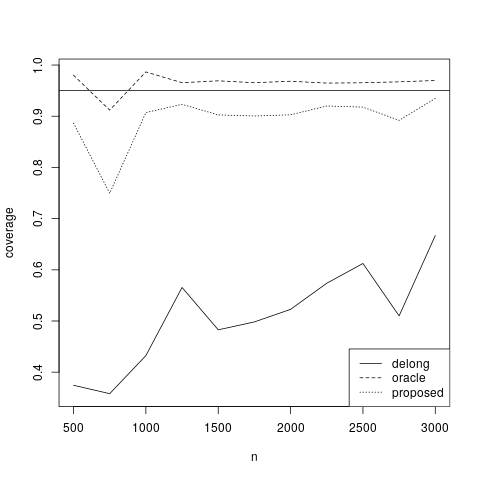
\includegraphics{./sim/lda/sim.png}
  \caption{Coverage simulation}
  \label{fig:1}
\end{figure}

\section{Discussion}
We have described a nonparametric method of estimating the index AUC
when the index coefficients are estimated from the same data on which
the AUC estimate is based. The method applies directly to testing for
the difference of index AUCs with estimated coefficients, when the two
AUCs are in the limit distinct. The method described above applies not
only to testing indexes based on nested data sets, perhaps the most
common situation, but more generally to a comparison of any correlated
AUCs with index coefficients estimated from the data, e.g., LDA versus
logistic. The main results also apply to discrete covariates, though
they were not considered among the examples here. The method is easily
extended to other differentiable functions of the data, not just an
index. For example, in the heteroskedastic LDA example considered
above, a common solution would be to use quadratic discriminant
analysis, though the marker in this case would be a quadratic function
of the covariates. An important limitation of the method described
here is that the coefficient estimation procedure have an influence
function, excluding many modern classification techniques.



\bibliographystyle{chicago}
\bibliography{delong.bib}

\end{document}
simulation:
## TODO:
## DONE--diff rather than just auc.
## full oracle (f-test) rather than just derivative oracle.
## maybe bad power in addition to bad fpr.
## coefs.lda should take x,g not x.0,x.1
## different strength of derivative
## maybe bootstrap estimator


other todo: logit normal model. it has been suggested no adj is
necessary. argument seems fallacious: based on logistic and lda coefs
converging to the same plim. but this assumes well specified
models. cannot be the both full and reducd models ar well
specified. weve shown that cofs proportional to probit coefs is
necessary for the deriv to vanish, regardless of the coefficient
esitmation procedure. so logit coefs for the reduced model would have
to be the same as probit coefs (in the plim), which isn't true?
